\icode{E-MD-SI-L3-261112-001}
 如图，在光滑水平面上有一质量为 \(m_1\) 的足够长的木板，其上叠放一质量为 \(m_2\) 的木块。假定木块和木板之间的最大静摩擦力和滑动摩擦力相等。现给木块施加一随时间 \(t\) 增大的水平力 \(F = kt\) (\(k\) 是常数)，木板和木块加速度的大小分别为 \(a_1\) 和 \(a_2\)。下列反映 \(a_1\) 和 \(a_2\) 变化的图线中正确的是\paren[]

 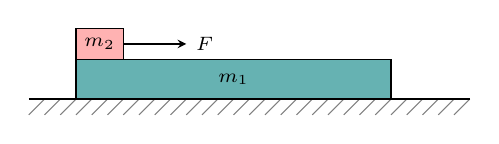
\begin{tikzpicture}[>=stealth,font=\scriptsize]
	\draw[fill=teal!60] (0,0) rectangle(4,.5)node[midway]{\(m_1\)};
	\draw[fill=red!30] (0,.5) rectangle(.6,.9)node[midway]{\(m_2\)};
	\draw[->] (.6,.7)--++(.8,0)node[right]{\(F\)};
	\foreach \x in {-.6,-.4,...,5}
		\draw[gray] (\x,-.2)--++(.2,.2);
	\draw[thick] (-.6,0)--(5,0);
 \end{tikzpicture}

 \begin{tikzpicture}[>=stealth,font=\scriptsize]
	\begin{scope}
		\draw[->,blue] (0,0)node[below left]{\(O\)}--(2.5,0)node[below]{\(t\)};
		\draw[->,blue] (0,0)--(0,2.5)node[right]{\(a\)};
		\draw[magenta] (0,0)--(1,1)coordinate(a) (a)--++(1,0)node[right]{\(a_1\)} (a)--++(60:1)node[right]{\(a_2\)};
		\node at(1.5,-.5){\normalsize\(A\)};
	\end{scope}
	\begin{scope}[xshift=3.5cm]
		\draw[->,blue] (0,0)node[below left]{\(O\)}--(2.5,0)node[below]{\(t\)};
		\draw[->,blue] (0,0)--(0,2.5)node[right]{\(a\)};
		\draw[magenta] (0,0)--(1,1)coordinate(a) (a)--++(1,0)node[right]{\(a_1\)} (a)--++(20:1)node[right]{\(a_2\)};
		\node at(1.5,-.5){\normalsize\(B\)};
	\end{scope}
	\begin{scope}[xshift=7cm]
		\draw[->,blue] (0,0)node[below left]{\(O\)}--(2.5,0)node[below]{\(t\)};
		\draw[->,blue] (0,0)--(0,2.5)node[right]{\(a\)};
		\draw[magenta] (0,0)--(1,1)coordinate(a) (a)--++(-40:1)node[right]{\(a_1\)} (a)--++(50:1)node[right]{\(a_2\)};
		\node at(1.5,-.5){\normalsize\(C\)};
	\end{scope}
	\begin{scope}[xshift=10.5cm]
		\draw[->,blue] (0,0)node[below left]{\(O\)}--(2.5,0)node[below]{\(t\)};
		\draw[->,blue] (0,0)--(0,2.5)node[right]{\(a\)};
		\draw[magenta] (0,0)--(1,1)coordinate(a) (a)--++(1,0)node[below]{\(a_1\)} (a)--++(0:1)node[above]{\(a_2\)};
		\node at(1.5,-.5){\normalsize\(D\)};
	\end{scope}
\end{tikzpicture}
\begin{answer}
	A\qquad 提示：
\end{answer}